\documentclass{article}

\usepackage[spanish]{babel}

\usepackage[letterpaper,top=2cm,bottom=2cm,left=3cm,right=3cm,marginparwidth=1.75cm]{geometry}

\usepackage{amsmath}
\usepackage{graphicx}
\usepackage{enumitem}
\usepackage{comment}
\usepackage{wrapfig}
\usepackage[colorlinks=true, allcolors=blue]{hyperref}

\title{AED Tema 2. Árboles I: Conceptos básicos}
\author{Martín González Dios 
\href{https://github.com/martindios}{\includegraphics[height=0.5cm]{github.png}}}

\begin{document}
\maketitle

\section{Conceptos básicos}
Árbol: \textbf{estructura de datos no lineal}, con una organización jerárquica y elementos homogéneos donde cada elemento puede tener varios elementos sucesores, pero un único elemento sucesor. \\
No puede haber rutas circulares en las conexiones de un árbol, de tal forma que sólo puede existir una única ruta desde cada nodo hasta la raíz. \\

Conceptos:
\begin{itemize}
    \item \textbf{Nodo}: cada uno de los componentes o elementos del árbol.

    \item \textbf{Ascendiente/antecesor}: nodo en un nivel superior dentro de la estructura jerárquica del árbol, accesible por ascenso repetido de hijo a padre.

    \item \textbf{Descendiente/sucesor}: nodo en un nivel inferior dentro de la estructura jerárquica del árbol, accesible por descenso repetido de  padre a hijo.

    \item \textbf{Nodo raíz}: nodo inicial del árbol. Se encuentra en el nivel superior de la estructura jerárquica del árbol, nivel 1.

    \item \textbf{Nodo hoja}: nodo terminal del árbol. Son todos aquellos que no tienen descendientes y se encuentran en los niveles más bajos de la estructura jerárquica del árbol, aunque pueden estar en distintos niveles del mismo.

    \item \textbf{Subárbol}: conjunto de nodos de un árbol que a su vez tienen estructura de árbol.

    \item \textbf{Nodo padre}: es el nodo ascendiente directo de sus subárboles. En un árbol cada nodo solo puede tener un padre, excepto el nodo raíz que carece del mismo.

    \item \textbf{Nodo hijo}: nodo descendiente directo de otro nodo. En un árbol cada nodo puede tener varios hijos.

    \item \textbf{Nodos hermanos}: dos nodos son hermanos si tienen el mismo padre.

    \item \textbf{Nodo interno}: es todo nodo que no es ni raíz ni hoja.

    \item \textbf{Camino}: secuencia de nodos donde cualquier par de nodos consecutivos son padre e hijo.

    \item \textbf{Longitud del camino}: número de nodos que forman el camino menos uno.

    \item \textbf{Rama}: cualquier camino desde el nodo raíz hasta un nodo hoja.

    \item \textbf{Nivel (profundidad) del nodo}: número de nodos que tiene el camino desde la raíz a dicho nodo.

    \item \textbf{Grado del nodo}: número de descendientes directos de dicho nodo (número de hijos).

    \item \textbf{Grado de un árbol}: máximo grado de sus nodos.

    \item \textbf{Peso}: número de nodos terminales u hojas del árbol.

    \item \textbf{Altura}: nivel más alto del árbol (número de niveles del árbol). La altura es igual al número de nodos que tienen la rama más larga del árbol.
\end{itemize}

\section{Árboles binarios}
\textbf{Definición}: árbol donde cada nodo tiene como máximo grado 2. \\
\textbf{Definición recursiva}: un árbol binario es un árbol vacío, o bien un nodo raíz con subárboles formados por árboles binarios a la izquierda y a la derecha. \\

Conceptos:
\begin{itemize}
    \item \textbf{Árbol binario equilibrado}: cuando la diferencia de altura entre los subárboles de cualquier nodo es como máximo una unidad.

    \item \textbf{Árbol binario lleno}: un árbol binario de altura h es lleno si tiene todas sus hojas a nivel h y todos los nodos que están en un nivel menor que h tienen cada uno 2 hijos. (Un árbol binario lleno es totalmente equilibrado)
\end{itemize}

Un árbol binario lleno es necesariamente completo. \\
Un árbol binario completo es equilibrado.

\section{Tipos de recorrido de un árbol binario}
\subsection{Recorrido en anchura}
Por niveles y, dentro de cada nivel, de izquierda a derecha.

\subsection{Recorrido en profundidad}

\begin{itemize}
    \item \textbf{Preorden}: raíz - izq - der. RID, notación prefija o notación polaca.

    \item \textbf{Inorden}: izq - raíz - der. IRD, orden normal de expresiones, orden simétrico u orden central.

    \item \textbf{Postorden}: izq - der - raíz. IDR o notación postfija de expresiones o notación polaca inversa.
\end{itemize}

\begin{figure}[h]
    \centering
    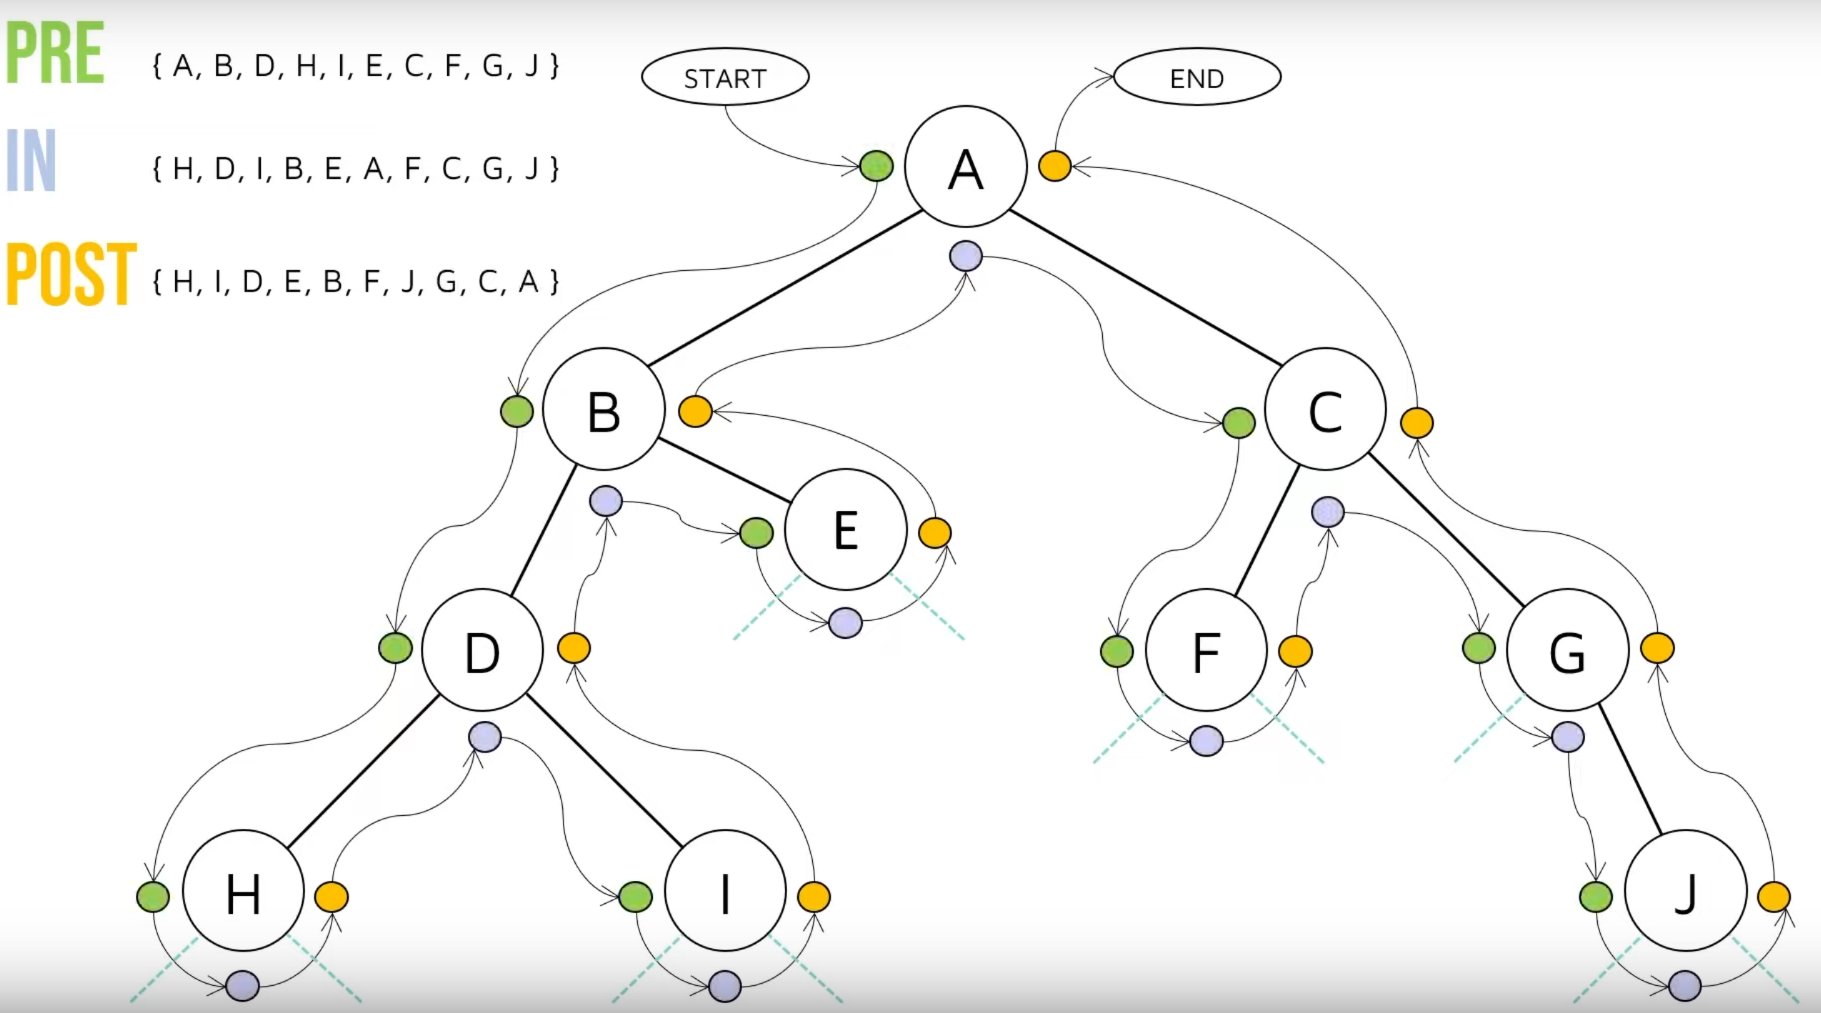
\includegraphics[width=0.85\textwidth]{img-t2/img_137_14.png}
\end{figure}

\newpage

\subsection{Recorridos no recursivos}
Usan estructuras auxiliares para almacenar puntero a los nodos del árbol.
\begin{itemize}
    \item \textbf{Recorrido en profundidad inorden no recursivo}. Usa una \textbf{pila} para almacenar los punteros a los nodos del árbol.
    \begin{enumerate}
        \item Se guardan los elementos izquierdos en la pila hasta llegar a un nodo sin hijo izquierdo.

        \item Se desapila el tope, se imprime y se inserta el hijo derecho.

        \item Se repiten los pasos 1 y 2 hasta que la pila esté vacía.
    \end{enumerate}

    \item \textbf{Recorrido en anchura no recursivo}. Usa una cola auxiliar para visitar los nodos por niveles.
    \begin{enumerate}
        \item Tomar el puntero raíz y ponerlo en la cola.

        \item Quitar el primer elemento de la cola, mostrar el contenido de dicho nodo y almacenar los punteros correspondientes a sus hijos izquierda y derecha.

        \item Repetir el paso 2 hasta que la cola esté vacía y el árbol recorrido.
    \end{enumerate}
\end{itemize}

\section{Árboles de expresión}
Los árboles binarios se utilizan para \textbf{representar expresiones en memoria}, esencialmente en compiladores de lenguajes de programación. \\

\textbf{Si suponemos operadores binarios}:
\begin{itemize}
    \item Los paréntesis no se almacenan (implícitos)
    \item Todos los operandos letras están almacenados en hojas.
    \item La raíz de cada subárbol es un operador.
\end{itemize}

Construcción a partir de una expresión en notación convencional (infija):
\begin{itemize}
    \item \textbf{Estructuras de datos auxiliares}:
    \begin{itemize}
        \item \textbf{Pila para almacenar punteros a los nodos de un árbol} (pila del árbol binario).
        \item \textbf{Pila para retener los operadores} temporalmente hasta que llegue el momento de incorporarlos al árbol. (pila de caracteres)
    \end{itemize}

    \item \textbf{Pasos}:
    \begin{enumerate}
        \item Cuando se lee un operando se crea un árbol de un nodo y se mete el puntero a él en la pila de punteros.

        \item Cuando se lee un operador: \\
        Si su prioridad $\leq$ que la del tope de la pila de operadores, se desapilan sucesivamente los operadores hasta que ya no se cumpla esta condición. \\
        Cada vez que se saca un operador de la pila también se sacan 2 punteros de la pila de punteros y se usan estos 3 elementos para crear un nuevo árbol. El puntero a este nuevo árbol se coloca en la pila de punteros. \\
        Finalmente, se introduce el operador en la pila.

        \item El proceso termina cuando se acaba la entrada y, en caso de que no esté vacía, se vacíe la pila de operadores.
    \end{enumerate}
\end{itemize}

\end{document}
